% Chapter 1

\chapter{绪论}
随着遥感技术的快速发展,我们能获得到越来越丰富的遥感观测数据。既有高分辨率的清晰图像,也包括低分辨率的鸟瞰图。这些图像从更宏观的视角为我们提供了许多有价值的数据。然而如何合理的使用这些图像数据,特别是从低分辨率图像中找出更多难以通过人类肉眼直接识别出的有效信息成为了一个重要的研究课题。在车辆计数等真实场景中,高分辨率图像虽然能提供丰富的细节,但有着获取成本高昂以及难以获取稳定连续的高频率数据的问题。本文在跨分辨率车辆计数数据集(Cross Resolution Vehicle Counting,CVRC)\cite{2022VehicleCountingVeryLowResolutionAerialImagesCrossResolutionSpatialConsistencyIntraresolutionTimeContinuity}上,设计了一种基于注意力机制\cite{vaswani2017attention}的深度学习U型网络模型,旨在提高跨分辨率遥感图像中隐含的空间和时间信息进行更丰富全面的表示,以进一步提升目标计数的准确性。
\section{研究背景与意义}
\subsection{高分辨率和低分辨率遥感图像简介}
在遥感领域,分辨率是用来描述遥感图像细节程度的一个重要指标,根据遥感卫星搭载的传感器不同,可以从多个维度进行描述,包括空间分辨率、时间分辨率、光谱分辨率和辐射分辨率。

空间分辨率指的是传感器能够区分的最小地面单元的尺寸,也称为地面采样距离(Ground Sample Disrance,GSD)。例如,如果一个卫星图像的空间分辨率是10米,那么图像上的一个像素代表真实世界中10米 x 10米的区域。空间分辨率越高(即图像中单个像素所代表的地面面积较小),图像的细节就越丰富,能够观察到更小的对象。

时间分辨率定义为重新访问并获取同一地点数据的所需的时间。重访周期是指卫星完成一个完整轨道周期所需的时间长度。因此,遥感系统第二次以相同视角对完全相同的区域进行成像的绝对时间分辨率等于该周期。然而,由于大多数卫星相邻轨道的成像带存在一定程度的重叠,并且这种重叠随着纬度的增加而增加,地球的某些区域往往会更频繁地重新成像。因此,传感器的实际时间分辨率取决于多种因素,包括卫星/传感器能力、测绘带重叠和纬度。

光谱分辨率描述的是遥感设备能够在电磁光谱中区分不同波长的能力。通常可以使用非常宽的波长范围(可见光和近红外)来区分广泛的类别,例如水和植被。其他更具体的类别,例如不同的岩石类型,就需要高光谱分辨率传感器在更精细的波长范围内进行比较才能将它们分开。

辐射分辨率描述的是遥感设备检测不同能级(亮度)的能力。不同传感器对电磁能大小的敏感度决定了辐射分辨率。传感器的辐射分辨率越精细,它对检测反射或发射能量的微小差异就越敏感。这对于分析物体的热特性、地表材料的性质等非常有帮助。


在讨论高分辨率(High Resolution, HR)图像和低分辨率(Low Resolution, LR)图像时,通常指的是空间分辨率的差异。空间分辨率的详细分类可以参照\cite{MultispectralImageAnalysisUsingObjectOrientedParadigm}:
\begin{enumerate}
    \item 低分辨率定义为地面采样距离为 30 m 或更大。
    \item 中分辨率的地面采样距离范围为 2-30 m。
    \item 高分辨率的地面采样距离范围为0.5-2 m。
    \item 极高分辨率的地面采样距离范围 <0.5 m。
\end{enumerate}

\subsubsection{高分辨率图像}
高分辨率图像通常指具有较高空间分辨率的图像,即图像中单个像素所代表的地面面积较小,能够显示更加精细的地面特征\cite{shimizu1983laser}。高分辨率图像使得用户可以观察到较小的地面对象,例如单个车辆、道路标线甚至是行人。虽然“高分辨率”这个术语没有绝对的定义,但在遥感领域,我们把空间分辨率小于1米(通常在0.3米到1米之间)的图像常被认为是高分辨率图像。目前我们可以使用的高分辨率遥感图像来源主要有:航空摄影(搭载高分辨率摄像机或低空高分辨率无人机拍摄的数据)和某些高性能的卫星遥感仪器,例如WorldView系列\cite{scitor2000project}、GeoEye、QuickBird等。
高分辨率图像中的精细地面特征信息,在城市规划、交通监控、农业监测(如作物健康分析)、详细的地物分类、灾害评估等领域都有广泛的使用。特别是在目标识别领域中,高分辨率的图像可以使用深度学习中多种模型和方法,具有很高的应用价值。


\subsubsection{低分辨率图像}

低分辨率图像指的是空间分辨率较低的图像,即图像中单个像素所代表的地面面积较大,只能显示较为粗糙的地面特征。低分辨率图像难以分辨较小的地面对象,但适合于观察大范围的地表变化。通常空间分辨率大于10米(如10米、30米或更大)的图像被认为是低分辨率图像。低分辨率图像主要来源于具有宽幅覆盖能力的卫星遥感仪器,如MODIS(具有数百米的空间分辨率)、Landsat系列(15米到30米分辨率)、Sentinel-2(10米到60米分辨率)等。图像中的大范围地表特征,在气候变化研究、大范围土地覆盖变化监测、环境监测、城市发展规划、海洋和大气研究等领域有着很高的应用价值。

对于不同任务,识别目标的大小不尽相同,对于图像分辨率的要求也随之变化。对于房屋的识别需要2-5米的分辨率,识别车辆需要1米以内的分辨率,行人的识别则需要0.3米或者更高。本文讨论的CVRC数据集是车辆识别数据集,将分辨率大于等于1米的图像认定为低分辨率图像,小于1米的视为高分辨率图像。对于目标识别以及目标计数领域来说,模糊的图像使得目标的轮廓极为模糊,稠密目标轮廓间的重叠更加大了模型识别的难度。


\subsubsection{重访周期与成本}

对于遥感卫星而言,其拍摄影像的分辨率是由传感器在地面采样的间隔决定的,即每个传感器探测元件在地面投影的大小,称为地面采样距离(Ground Sample Disrance,GSD)。在理想状况下,地面采样距离可以通过下式计算:
\begin{equation}
    GSD = {\frac{dR}{f}} \label{eq:GSD}​​​​
\end{equation}
其中\(d\)为传感器探测元件的宽度,\(R\)为传感器距离地面高度,\(f\)为光学系统焦距.

通过万有引力定律和开普勒第三定律,可推出遥感卫星绕地球旋转的周期与轨道半径之间的关系。
\begin{equation}
    T = 2\pi \sqrt{\frac{r^3}{G (M + m)}} \label{eq:T}​​​​
\end{equation}

由式\ref{eq:GSD}和式\ref{eq:T},可以分析高低分辨率图像拍摄卫星的轨道条件。高分辨率图像一般由低轨卫星拍摄,具有较小的轨道半径和周期。同时也因此具有较小的视场(the field of view, FOV)较小。高分辨率图像辨率卫星通常使用任务驱动模式进行地球观测。这意味着,如果不提前提交观测任务,一颗卫星需要6个月才能完成全球覆盖,获得特定区域的图像的重访周期相当长。此外,高分辨率图像非常昂贵,例如 WorldView-3 的价格为34美元/平方公里。作为对比,低分辨率卫星的往往运行在更高的轨道上,虽然空间分辨率有所降低,但视场较大。因此获得同一地点重访周期要短得多,例如 PlanetScope 卫星每天重访一次,价格也低得多,为 1.8 美元/平方公里。不同分辨率卫星的拍摄成本和覆盖周期如下表\ref{tab:cost}所示。
\begin{table}[h]
    \centering
    \caption{不同分辨率卫星拍摄成本及覆盖周期}
    \label{tab:cost}
    \begin{tabularx}{\textwidth}{CCCCC}
      \toprule
      名称 & 分辨率 & 重访周期& 全球覆盖周期 & 花费 \\
      \midrule
      WorldView-3    & 0.3m  &4.5天 &6个月&34美元/$km^2$\\
      GeoEye-1    & 0.4m  &4天 &6个月&29.5美元/$km^2$\\
      SuperView-    & 0.5m  &4天 &6个月&23美元/$km^2$\\
      QuickBird    & 0.6m  &7天 &6个月&17.5美元/$km^2$\\
      Spot 6/7    & 1.5m  &2天 &1个月&5.75美元/$km^2$\\
      PlanetScope    & 3m  &小于1天 &小于5天&1.8美元/$km^2$\\
      RapidEye    & 5m  &1天 &小于1个月&1.28美元/$km^2$\\
      \bottomrule
    \end{tabularx}
\end{table}

\subsection{研究意义}
单独依靠低分辨率图像进行目标计数是十分困难的,而仅通过高分辨率图像进行目标计数,不仅花费巨大,同时还需要面对连续监控数据的缺失。如何通过低成本且具有时间连续性的低分辨率图像进行目标计数及实时监测就成为解决问题的关键。本文提出的方法通过少量高分辨率图像的辅助,在时间连续的低分辨率图像上实现目标计数,具有很高的应用价值。该方法不仅局限于目标计数,更好地利用了低分辨率图像中蕴含的模糊信息,在稠密车流人流识别、智慧城市设计等领域也有很高的应用潜力。

\section{国内外研究现状}
\subsection{跨分辨率遥感影像目标计数现状}
高分辨率图像计数主要有三类方法。基于检测的计数方法通过识别出具体的物体位置来进一步计数。基于回归的计数类方法通过学习出图像与图像中对应物体的数目的对应关系,从而估计出目标数目。基于密度图的计数方法生成图像对应的密度图,通过密度分布求和计算出最终的数量估计。

\subsubsection{基于检测的计数方法}
基于检测的目标计数是目标检测下的一个分支。目标检测作为计算机视觉的一个主要研究方向,主要研究的是如何利用计算机视觉技术识别特定对象并确定其大小和位置。目前随着深度学习技术的发展,利用神经网络进行目标检测已经成为主流方案。主要的目标检测算法包括RCNN系列\cite{girshick2014rich,girshick2015fast,ren2015faster}、SSD\cite{liu2016ssd}、YOLO系列\cite{redmon2016you,redmon2017yolo9000}等。应用这些方法,可以通过先检测出目标位置,再进一步计数从而满足目标计数的需求。

这些方法虽然在目标识别上极为准确,但对数据集的质量和分辨率要求非常高。它们依赖于精确的边界标注,通常需要大量的人工标注后的高分辨率图像以确保检测的准确性。但是在CVRC数据集中,只包含少量具有人工标注的高分辨率图像,其余大量数据均为低分辨率图像。这些低分辨率图像上的目标识别难度大,以至于即便是人工也难以准确识别出具体的车辆数目。在这种情况下,即使是研究人员也通常需要借助同一地点不同时间拍摄的高分辨率图像来辅助识别。

除此之外,目标检测算法在处理极度拥挤或遮挡严重的环境时也面临挑战。为了解决这些问题,一些研究开始集中于开发更加鲁棒的检测算法,这些算法可以更好地处理低质量图像和复杂场景、进一步地,为了降低对高分辨率标注数据的依赖,研究人员也在探索半监督和弱监督学习方法\cite{karimijafarbigloo2023self}。这些方法通过利用少量标注数据与大量未标注数据,能够有效地提升模型的泛化能力和减少人工标注的工作量。此外,迁移学习技术\cite{cheng2021transfer}也被广泛使用,先在高分辨率图像上训练得到的模型,使用该模型在低分辨率图像的进行微调来提高目标检测性能。


\subsubsection{基于回归的计数方法}
基于回归的计数方法\cite{2022Crowddetectionanalysissurveillancevideosusingdeeplearning,2008PrivacypreservingcrowdmonitoringCountingpeoplepeoplemodelstracking,2009BayesianPoissonRegressionCrowdCounting}从深度神经网络提取的特征中直接进行数目的回归估计,常常用于处理目标密集、相互遮挡严重的场景,如人群计数。贝叶斯泊松回归模型\cite{2009BayesianPoissonRegressionCrowdCounting} 考虑数据的内在波动性,为估计值提供置信区间,从而增强模型在各种拥挤场景下的鲁棒性。隐私保护人群监控\cite{2008PrivacypreservingcrowdmonitoringCountingpeoplepeoplemodelstracking} 通过模糊处理技术确保在计数过程中不泄露个人信息,适用于对隐私要求严格的应用场景。Shi 等人\cite{2018CrowdCountingDeepNegativeCorrelationLearning}设计的模型通过训练多个回归器并引入负相关性来提高总体预测的准确性和泛化能力。这些方法的共同点在于它们都通过深入分析和学习图像特征来直接预测目标数量,无需进行繁琐的目标检测和识别,从而在处理极度拥挤场景时显示出显著优势。
\subsubsection{基于密度图的计数方法}
基于密度图的计数方法通过估计目标区域的目标密度,从而计算出数量估计。为了生成像素级的密度估计图像,语义分割中的许多方法也被研究人员用以参考。主要的语义分割模型包括全卷积网络(FCN)\cite{long2015fully}、U-Net\cite{ronneberger2015u}、SegNet\cite{badrinarayanan2017segnet}、DeepLab\cite{chen2014semantic,chen2017deeplab,2017RethinkingAtrousConvolutionSemanticImageSegmentation}系列、Mask R-CNN\cite{he2017mask}和Attention U-Net\cite{oktay2018attention}。目前主要的密度图估计方法包括CSRNet\cite{li2018csrnet}、MCNN\cite{2016SingleImageCrowdCountingMultiColumnConvolutionalNeuralNetwork}和CrowdNet\cite{boominathan2016crowdnet}。这些方法通过使用不同架构的卷积神经网络来处理稠密场景下的复杂视觉信息,以精确地估计高密度目标如人群的密度密度。CSRNet 采用了带扩张卷积的深层网络,能够在保持有效感受野的同时,更好地捕获人群密集区域的细节信息。而MCNN 通过多列卷积结构来适应不同尺度的人群密度,这对于处理不同距离拍摄的人群图像特别有效。CrowdNet,结合浅层和深层网络架构,分别识别高低分辨率中的特征信息,来有效捕捉人群图像中的多尺度信息,从而使得模型能够在复杂的人群场景中更准确地估计人数。

尽管基于密度图的方法在稠密目标数量估计问题中显示出了优越的性能,它们依然面临一些挑战。首先,这些方法往往需要大量标记数据来训练深度学习模型,而高质量的标记数据获取成本较高,尤其是在极端环境下的人群场景。此外,这些模型在遇到极端天气条件或光线不佳的情况时,性能可能会显著下降。Liu等人\cite{2018CrowdCountingusingDeepRecurrentSpatialAwareNetwork} 提出了一种通过增强数据的方法来提升模型在不同环境下的鲁棒性,该方法通过模拟不同天气和光照条件下的图像,增强了模型对这些变化的适应性。另外,Boominathan 等人\cite{boominathan2016crowdnet} 则关注模型泛化能力的提升,他们通过引入域自适应技术减少了模型对特定数据集的依赖,从而提高了模型在未见过场景中的表现。

上述几种方法在大型高分辨率图像数据集下均有着不错的表现。但对于CRVC数据集来讲,由于高分辨率图像的稀缺,这些方法不能很好的完成CRVC数据集中的任务。如何通过少量高分辨率图像信息指导改进大量低分辨率图像上估计的结果成为模型设计的关键。

\subsection{跨分辨率车辆计数数据集}
跨分辨率车辆计数数据集\cite{2022VehicleCountingVeryLowResolutionAerialImagesCrossResolutionSpatialConsistencyIntraresolutionTimeContinuity} (CRVC)收集了日本常陆那珂港的 192 张极低分辨率图像和 8 张高分辨率图像,日期范围为 2016 年至 2019 年。\begin{figure}[h]
    \centering
    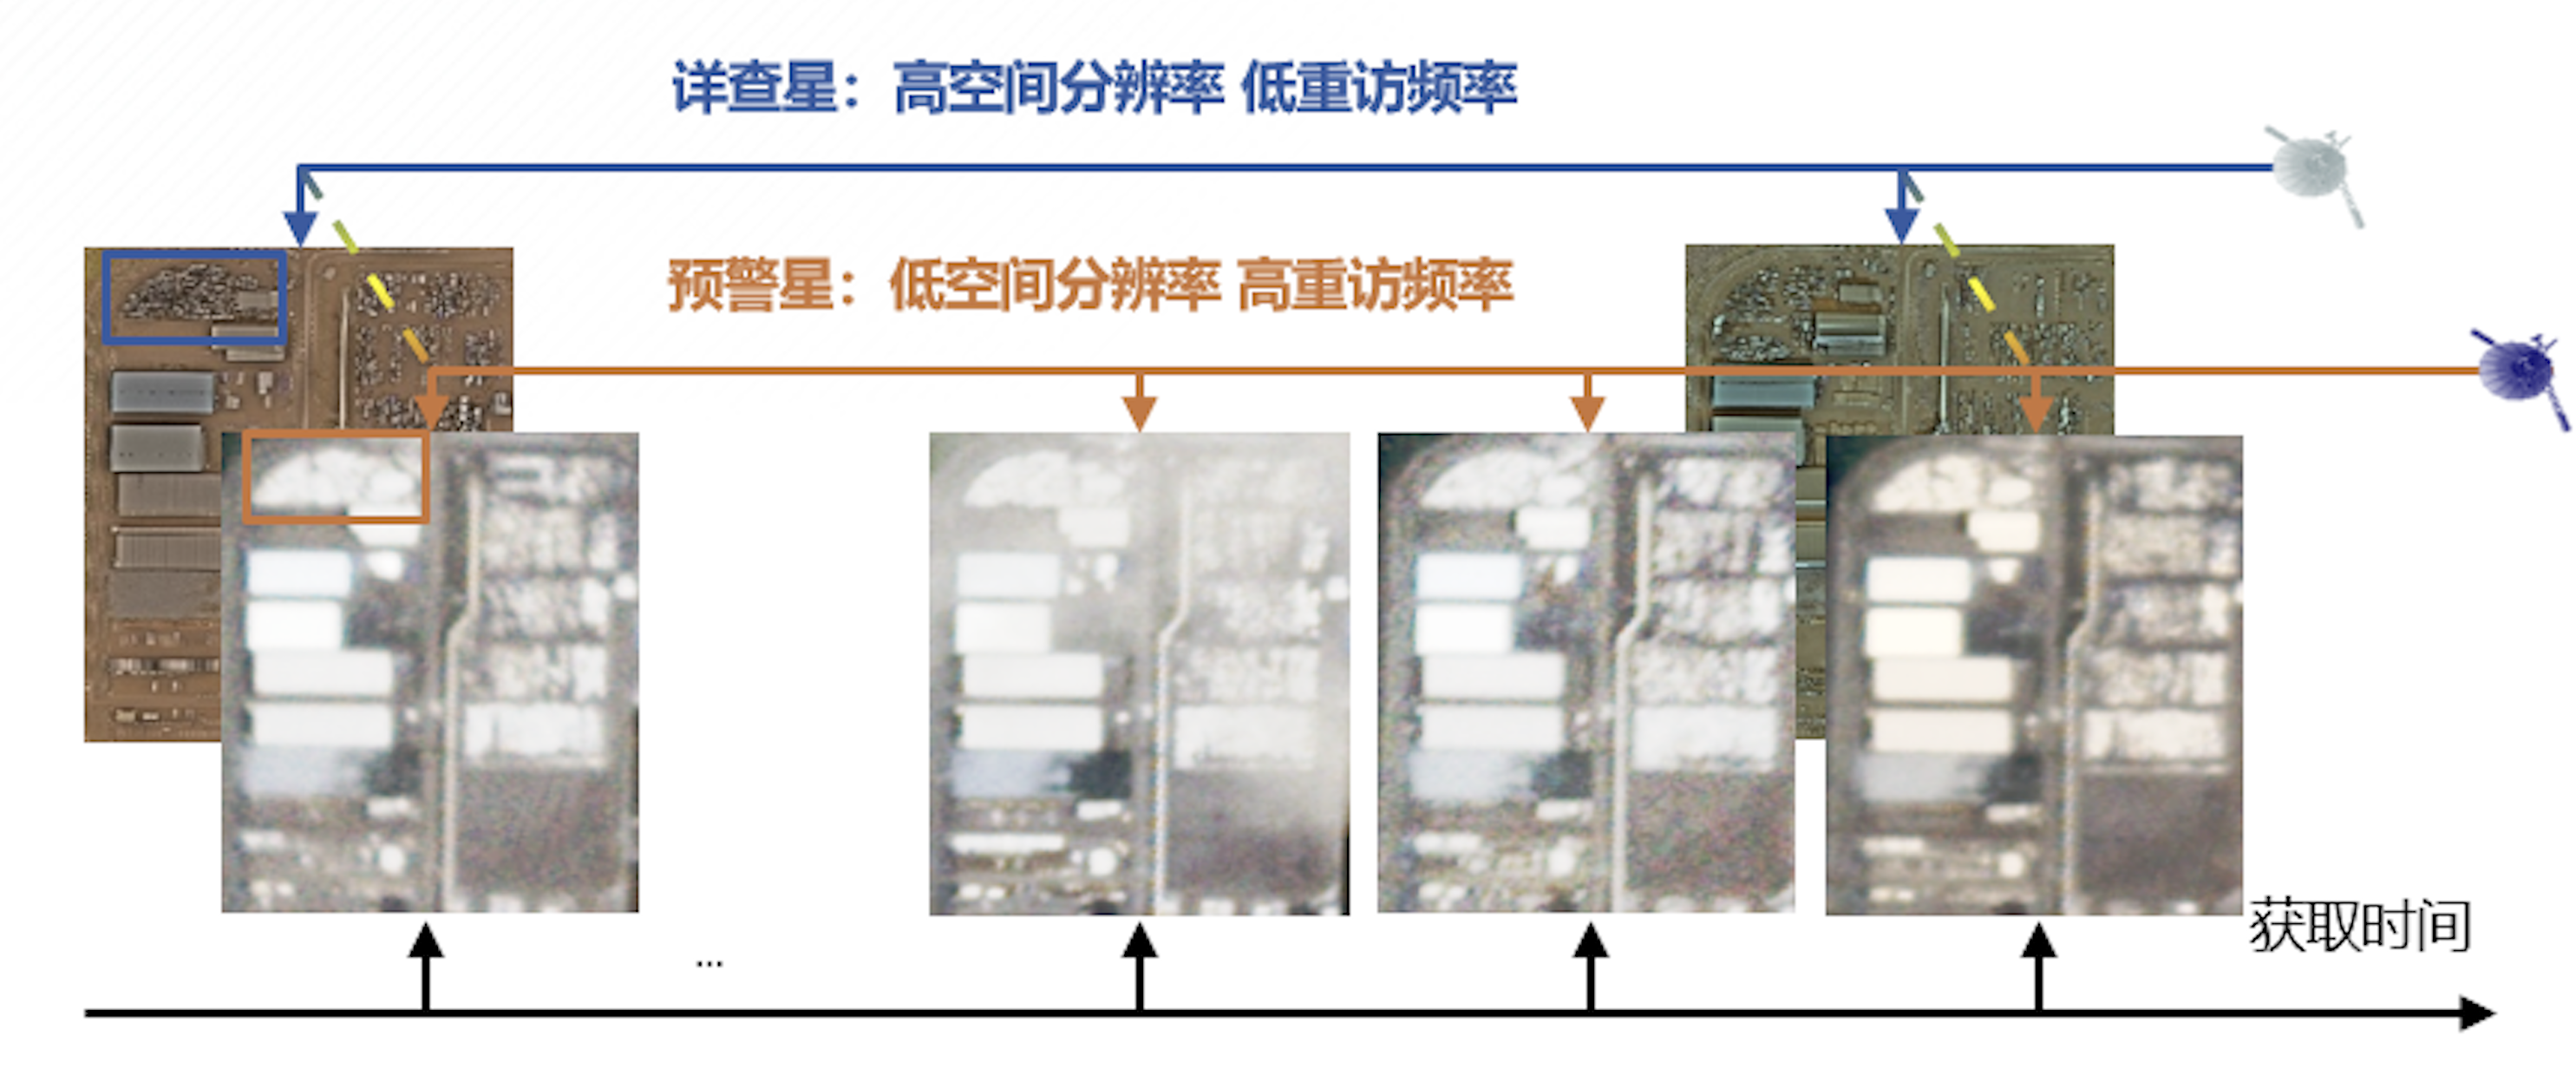
\includegraphics[width=\textwidth]{dataset.png}
    \caption{数据集概览}
    \label{fig:dataset}
\end{figure} 

其中LR 图像是www.planet.com 下载的,由 PlanetScope 卫星拍摄,地面分辨率为每像素 3m。为了起到监督作用,HR 图像是在根据相应 LR 图像的日期选择的,这些图像是从 WorldView 捕获的,地面分辨率为每像素 30 厘米。


\subsubsection{数据集分析}  
\begin{figure}[H]
    \centering
    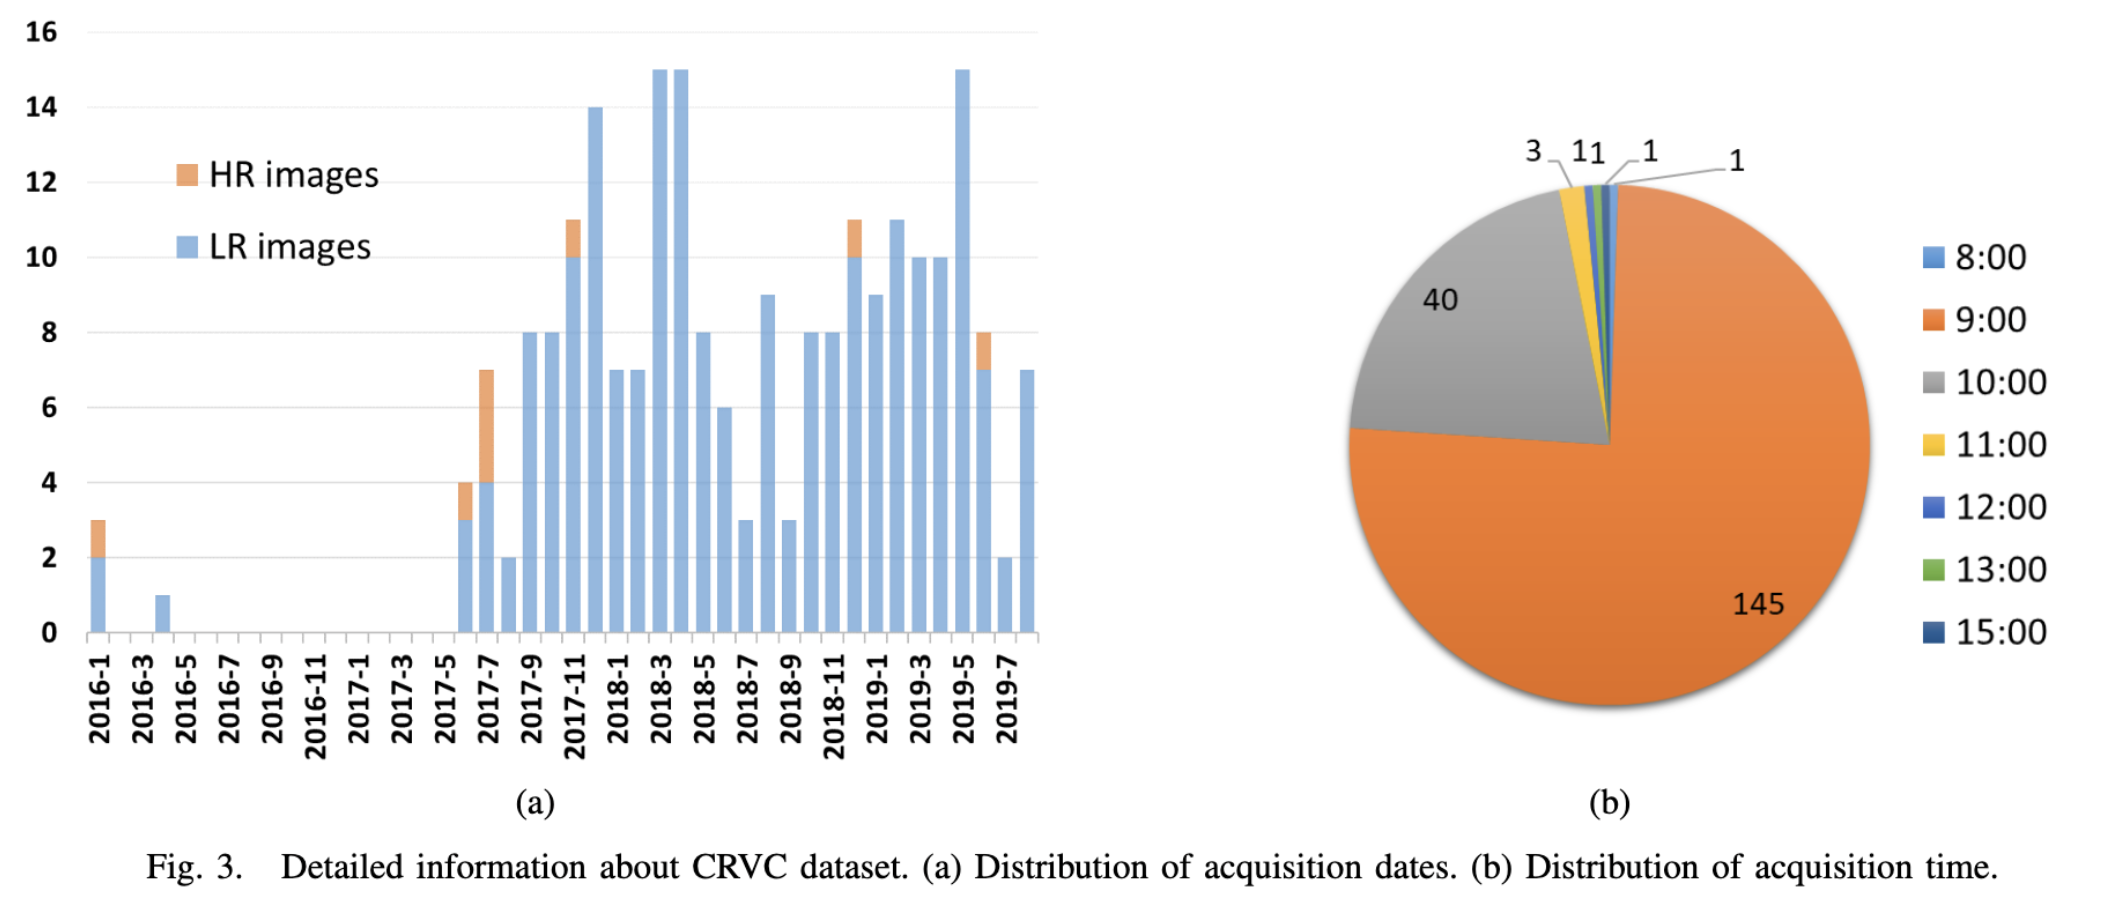
\includegraphics[width=\textwidth]{CRVCtime.png}
    \caption{数据的日期和时间分布}
    \label{fig:CRVCtime}
\end{figure}
图 ~\ref{fig:CRVCtime} 显示了数据集中LR和HR图像采集的日期和时间分布。可以观察到,数据的分布并不平均,主要集中在2017年5月至2019年7月之间。就8张高分辨率图像的日期而言,它们之间的时间间隔最小为 6 天,最大为 17 个月。 如表格~\ref{tab:date}中数据所示,HR 图像和相应 LR 图像之间的采集时间并不完全一致,平均采集时间差异为 39 分钟。在这种情况下,我们认为短时间内的HR和LR图像中的车辆数目一致。这一假设和实际情况相符并大大降低了建模难度。 
\begin{table}[h]
    \centering
    \caption{HR和LR图像的获取日期与时间}
    \label{tab:date}
    \begin{tabularx}{\textwidth}{CCCC}
      \toprule
      日期 & HR拍摄时间 & LR拍摄时间  \\
      \midrule
      4th January, 2016    & 10:56  &10:36\\
      26th June, 2017      &10:24   & 9:34\\
      2nd July, 2017       &10:20   & 9:36\\
      9rth July, 2017      &10:34   & 9:44\\
      15th July, 2017      &10:30   & 9:41\\
      9th November, 2017   &10:25   & 9:42\\
      19th December, 2018  &10:46   & 9:56\\
      6th June, 2019       &10:35   &10:29\\
      \bottomrule
    \end{tabularx}
\end{table}


\subsubsection{高分辨率图像处理}  
为了进行计数任务,该数据集在HR图像上标注了车辆的边界及类别。HR图像上标注框的数量作为对应日期的LR图像的真值。标注的边界则作为停车场位置的空间提示信息。该数据集中总共注释了 37852 个车辆实例,包含四类车辆,包括轿车、小型卡车、大型卡车和起重机(图~\ref{fig:vehicle})。不同类别的车辆在尺寸形状上有着很大的不同,分类计数有助于提升计数质量。  各类车辆数量极不平衡,分别为轿车35844辆、小型货车737辆、大型货车1211辆、起重机60辆。 
\begin{figure}[h]
    \centering
    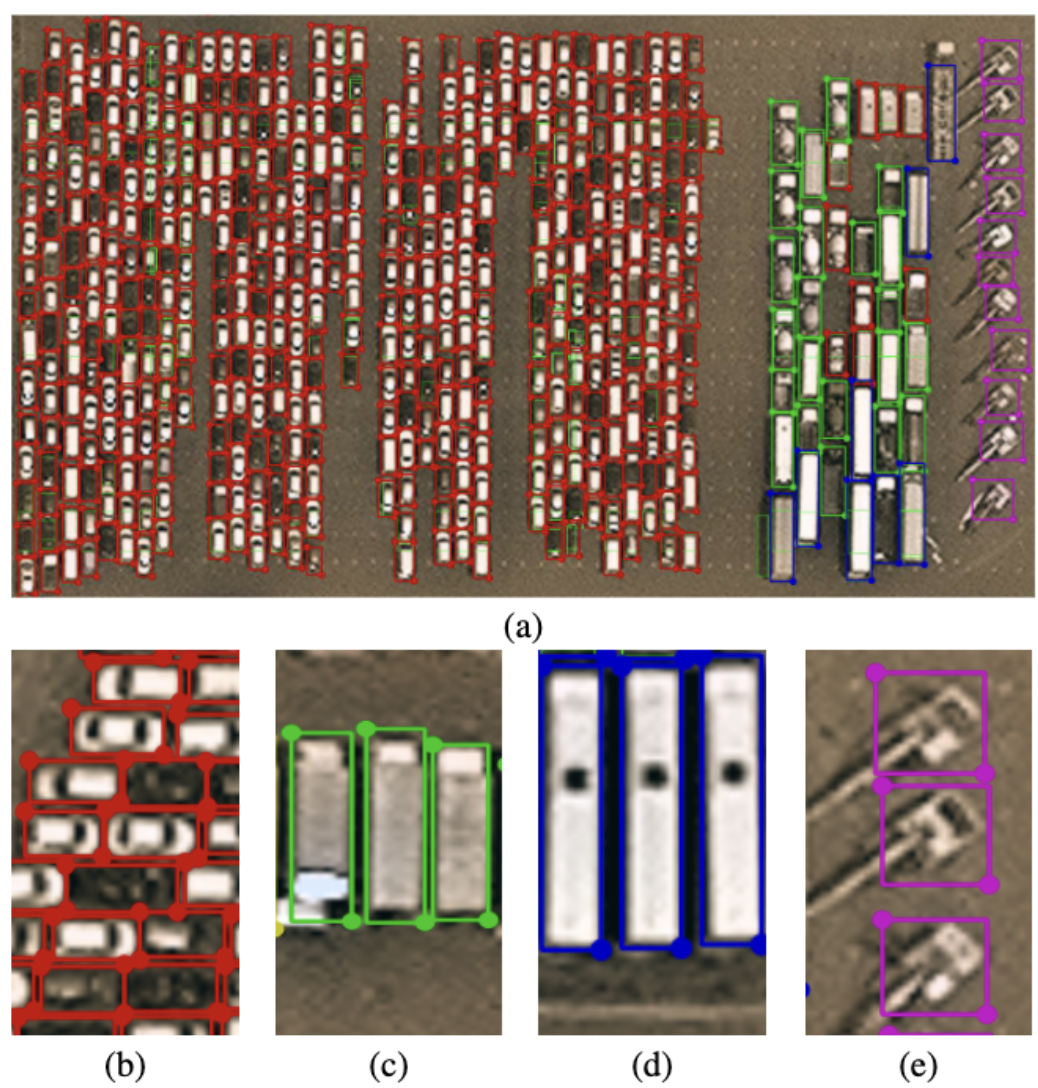
\includegraphics[width=0.5\textwidth]{vehicle.png}
    \caption{HR图像车辆标注及分类}
    \label{fig:vehicle}
\end{figure}

\subsubsection{低分辨率图像处理}  
数据集中共包含192张低分辨率图像。这些图像在2016至2019年之间被采集,主要分布在2017年6月至2019年8月之间,其中61.5\%的采集间隔在两天以内。如图~\ref{fig:CRVCtime}所示,低分辨率图像的采集时间均为日间,大部分图像拍摄于上午9点到10点。我们可以认为这些图像具有相似的拍摄条件。
不同于高分辨率图像,低分辨率图像的标注要困难的多。因为难以在低分辨率的条件下辨认清晰的车辆轮廓,所以标注车辆覆盖率是一个更可行的方法。由于低分辨率图像的视场较大,车辆区域只占图像中很小的一部分。因此先在HR图像中划出9个区域(图~\ref{fig:9parkHR}),在LR图像中对应位置进行覆盖率估计(图~\ref{fig:9parkpair})。
\begin{figure}[h]
    \centering
    \begin{subfigure}{0.45\textwidth}
        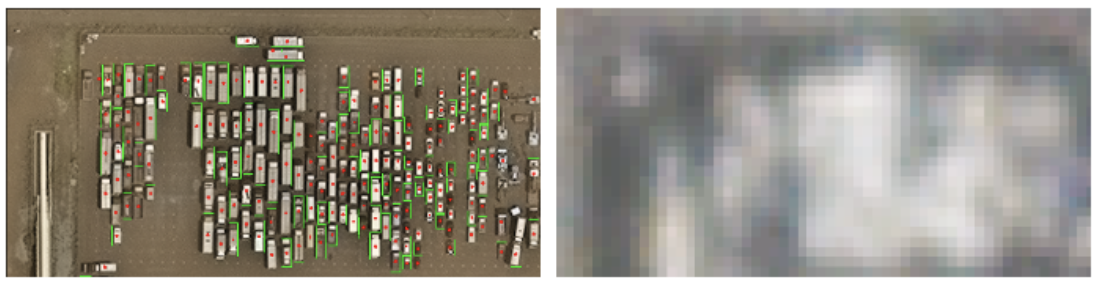
\includegraphics[width=\linewidth]{9parkpair.png}
        \caption{区域2对应的HR和LR图像}
        \label{fig:9parkpair}
    \end{subfigure}
    \begin{subfigure}{0.45\textwidth}
      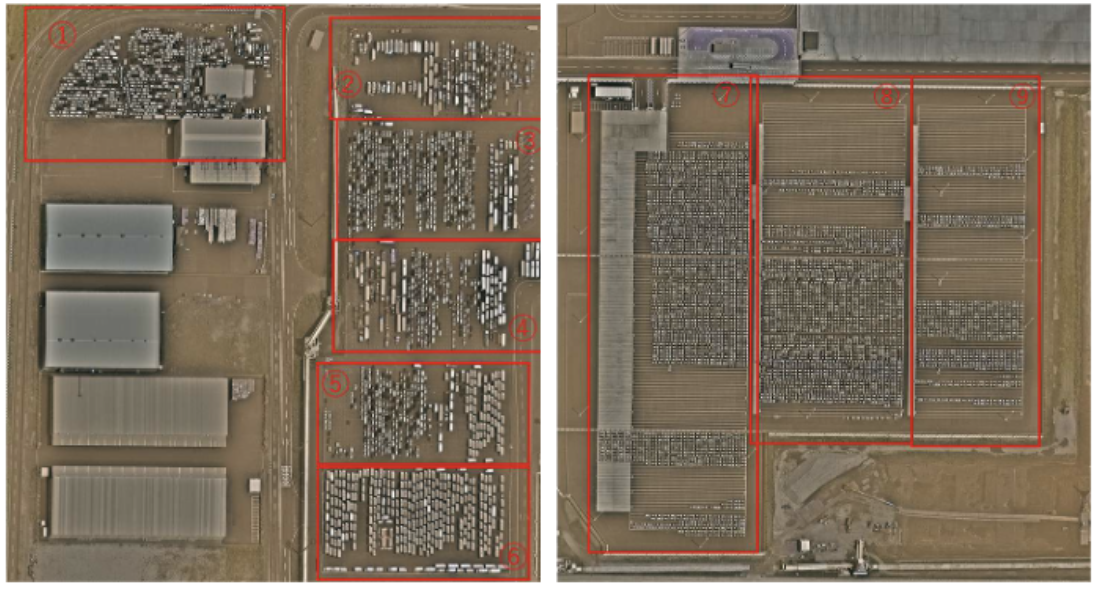
\includegraphics[width=\linewidth]{9parkHR.png}
      \caption{9个停车区域}
      \label{fig:9parkHR}
    \end{subfigure}\quad % 添加一些间隔
    
\end{figure}

% \begin{figure}[h]
%     \centering
%     \begin{subfigure}{\textwidth}
%         \centering
%         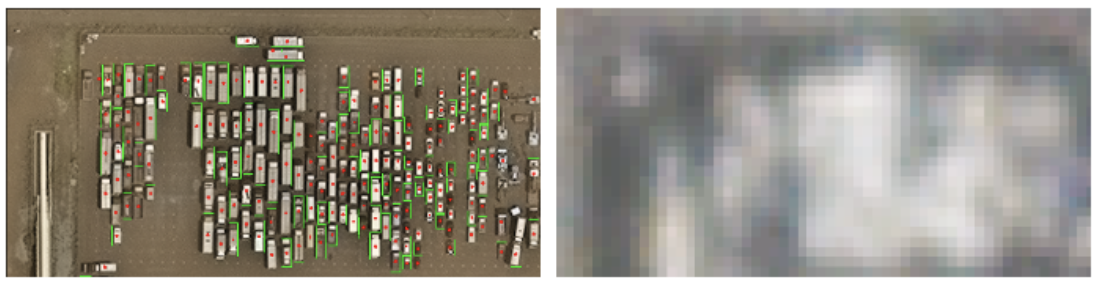
\includegraphics[width=0.6\linewidth]{9parkpair.png} % 调整宽度以适应你的需求
%         \caption{区域2对应的HR和LR图像}
%         \label{fig:9parkpair}
%     \end{subfigure}
    
%     \begin{subfigure}{\textwidth}
%       \centering
%       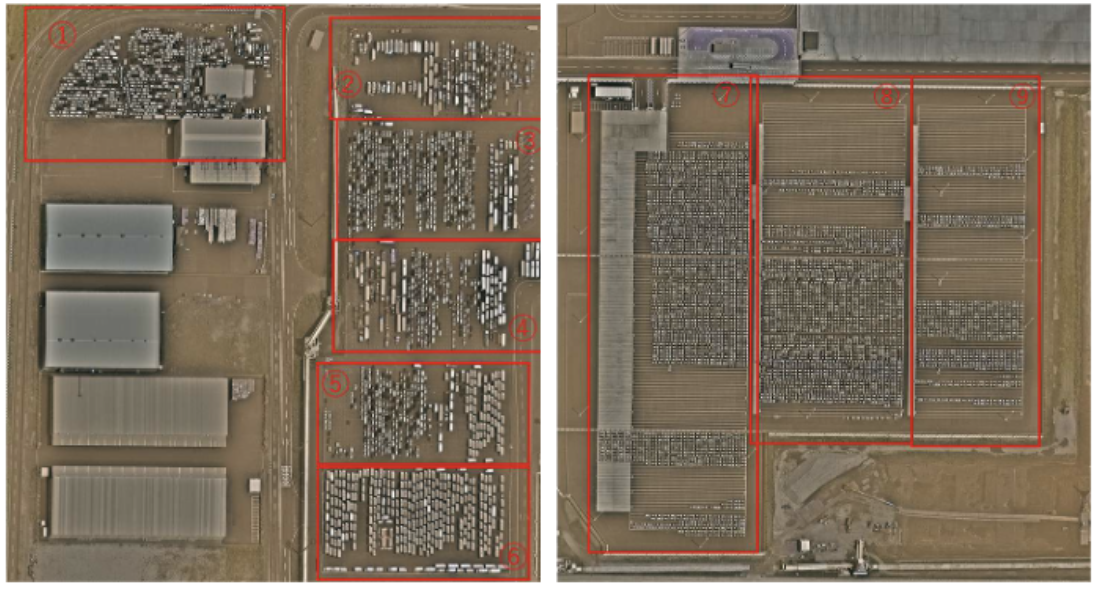
\includegraphics[width=0.6\linewidth]{9parkHR.png} % 调整宽度以适应你的需求
%       \caption{9个停车区域}
%       \label{fig:9parkHR}
%     \end{subfigure}
    
%     % \caption{这是两个子图的总标题。}
%     \label{fig:combinedfigure}
% \end{figure}



低分辨率图像可以分为两类,有对应高分辨率图像的和没有对应高分辨率图像的。对于前者而言,直接从对应高分辨率标注结果中计算覆盖率即可。那些没有HR图像对应的LR图像则由多名专家进行视觉标注并取平均值。


\subsubsection{数据集特性分析}  
通过上述对数据集的分析,我们可以看到高分辨率图像和与其对应的低分辨率图像之间间隔时间不大,同时对应的是同一位置。因此我们可以认为在它们上进行的目标计数结果应当也相同。两者所映射的空间信息应该具有一致性,这也给后续处理方法提供了思路。如何应用高分辨率图像信息指导改进低分辨率图像上估计的结果成为提高估计精度的关键节点之一。

同时单一的低分辨率图像很难得出合理的目标计数估计,然而由于低分辨率遥感图像的短重访周期,我们能得到一段连续的低分辨率图像。比较相邻图像间的变化或者从多个图像间进行学习,可以补充那些单张图像因低分辨率造成的信息缺失。图像间的时间连续性也是指导改进图像计数估计结果的关键因素。

\section{研究目标与内容}
\subsection{研究目标}
\begin{enumerate}    
    \item 跨分辨率车辆计数算法的开发:开发一种新的基于深度学习的车辆计数算法,该算法能够有效利用有限的高分辨率图像来指导低分辨率图像中的车辆计数。
    \item 探究高效利用数据集中空间一致性和时间连续性信息的方式:探究同一时刻高分辨率与低分辨率图像间的空间一致性和连续低分辨率图像间的时间连续性的高效利用方式。研究不同分辨率图像对算法效果的具体影响。
    \item 探究注意力机制在跨分辨率目标计数的应用:探索注意力机制在提高跨分辨率车辆计数准确性中的应用,尤其是如何通过注意力机制来增强模型综合多种特征表示的能力。
\end{enumerate}

\subsection{研究内容}
\begin{enumerate}
    \item 研究背景与意义分析:分析相关遥感技术的发展背景,高分辨率与低分辨率遥感图像的特点及其在车辆计数中的面临困难和挑战。梳理了当前目标检测、语义分割、基于回归和密度图的计数方法等方面的研究进展,特别关注跨分辨率图像处理及车辆计数领域的最新研究成果。
    \item 跨分辨率车辆计数数据集分析:对CRVC数据集进行分析调研,了解其数据组成分布以及数据中隐含的性质的分析及建模。
    \item 基于注意力机制的车辆计数模型设计:设计并实现一种新的基于注意力机制的深度学习模型,用于提高跨分辨率遥感图像车辆计数的准确性。
    \item 算法的性能评估及优化:在CRVC数据集上评估设计算法的性能,进行消融实验,并与现有的车辆计数方法进行比较。进一步优化算法,以达到更高的计数准确性和更好的泛化能力。
\end{enumerate}

\section{章节安排}
第一章为绪论,整体介绍研究背景及研究内容。第二章为相关工作分析,分析了几种的计数方法在跨分辨率图像计数数据集上的局限性,同时介绍了几种对于本文设计有所启发的研究工作。第三章介绍了基于注意力机制的跨分辨率遥感影像计数方法,详细解释了基于注意力机制的深度学习网络设计细节。第四章设计了多组实验从分割精度、覆盖率估计和回归计数结果这三个方面测试了模型的性能。第五章对本设计做出总结和展望。
